% Chapter 1

\chapter{Introducción} % Main chapter title

\label{Chapter1} % For referencing the chapter elsewhere, use \ref{Chapter1} 

%----------------------------------------------------------------------------------------

% Define some commands to keep the formatting separated from the content 
\newcommand{\keyword}[1]{\textbf{#1}}
\newcommand{\tabhead}[1]{\textbf{#1}}
\newcommand{\code}[1]{\texttt{#1}}
\newcommand{\file}[1]{\texttt{\bfseries#1}}
\newcommand{\option}[1]{\texttt{\itshape#1}}

%----------------------------------------------------------------------------------------

\section{Tema principal}

\ttitle.


%----------------------------------------------------------------------------------------

\section{Introducción}

Los campos de \emph{\gls{machine learning}} (aprendizaje de máquinas o aprendizaje artificial) y \textit{\gls{deep learning}} (\gls{aprendizaje profundo}) \parencite{lecun2015deep} no son nuevos, pero se han vuelto gran sensación en los últimos años, cada vez ganando más popularidad. Los primeros conceptos desarrollados en el campo tienen décadas de antigüedad. La primer \gls{red neuronal} --- la base del modelo a utilizar en este trabajo y la base del campo de Deep Learning --- fue planteada en los años 80 \parencite{werbos1982applications}. ¿Qué ha cambiado entonces en los últimos años, que ha generado una explosión en el área? La disponibilidad de los datos y la accesibilidad a poder computacional \parencite{jordan2015machine}. Con el surgimiento y la penetración cada vez más alta del internet se han abierto las puertas a cantidad de datos nunca antes vista.

La revolución de los datos ha llevado a la comunidad científica y a las industrias a recolectar grandes cantidades de datos e información y organizarlos de forma que se puedan interpretar y obtener valor de la misma.

Los sistemas de Deep Learning necesitan pasar por una fase de aprendizaje (comúnmente llamada fase de \gls{entrenamiento}) y estos modelos tienen la característica de necesitar cantidades masivas de datos para generalizar bien lo aprendido. Esto, combinado con la explosión de datos, ha llevado a que las técnicas tengan un surgimiento en todas las áreas de software, mostrando mucha promesa en algunos campos en específico como \gls{cv} \parencite{hoo2016deep} y en \gls{nlp}.

Conforme ha avanzado el campo se ha determinado que para algunas tareas en específico no se cuenta con la cantidad necesaria para obtener un modelo competente. Esto ha llevado al desarrollo de una técnica llamada transfer learning, que permite utilizar conocimiento previamente obtenido al resolver una tarea general y aplicarlo a una tarea relacionada mediante proceso de ajuste. Esta fase requiere de una cantidad de datos considerablemente menor, comparado con tener que entrenar un modelo completamente desde cero.

La técnica de transfer learning ha permitido muchos avances en el área de \gls{cv} específicamente \parencite{hoo2016deep}. Este trabajo intenta mostrar que se puede aplicar este concepto en un área distinta, puntualmente el campo de NLP, específicamente en el proceso de \gls{perfilamiento de autores}.

\section{Hipótesis}

\textbf{La aplicación de transfer learning en la tarea de perfilamiento de autores provee una ventaja en desempeño medible.} Se desglosa en los siguientes aspectos:

\begin{itemize}
\item \textbf{Aplicabilidad de deep learning en la tarea}. La hipótesis se basa en el hecho de que conceptos de deep learning sean aplicables a tareas del campo de NLP. En el campo de NLP se ha tenido mucha duda si deep learning tiene la capacidad de penetrar el campo con soluciones eficaces.

\item \textbf{Transfer learning provee ventaja de desempeño en la tarea}. El hecho de mostrar que hay una ventaja, implica medir de forma empírica los resultados obtenidos por diferentes técnicas. Con este fin se utilizarán resultados publicados por investigadores de este campo y se usarán las mismas métricas para que los resultados sean directamente comparables.

\item \textbf{Diferencia en cantidad de datos disponibles}. Se debe fundamentar que la cantidad de datos necesaria para el uso de deep learning es más elevado del que se necesita si se utiliza transfer learning.
\end{itemize}

%-----------------------------------------------------------------------------------------

\section{Objetivo General}

Aplicar conceptos del estado del arte a un problema que ha recibido poca atención en el área de \gls{procesamiento de lenguaje natural} (NLP), por sus siglas en inglés). Lo anterior con el propósito de mostrar la capacidad de las redes neuronales recurrentes (\glspl{rnn}) y \textit{\gls{transfer learning}} en la tarea específica.

\subsection{Objetivos específicos}

\begin{itemize}
\item Ser pionero en la aplicación de transfer learning en la tarea específica de perfilamiento de autores en el área de procesamiento de lenguaje natural.
\item Exponer las ventajas y desventajas de utilizar esta tecnología en esta subtarea.
\item Exponer como caso de uso la utilidad de esta aplicación en distintas áreas, como en el mercadeo.
\item Contribuir a la academia con los resultados obtenidos
\end{itemize}

%----------------------------------------------------------------------------------------

\section{Planteamiento del problema}

En el área de NLP han existido técnicas poderosas por décadas que abusan de algunas suposiciones que no siempre reflejan la realidad y se basan en simples métodos estadísticos que asignan valores a características del texto \parencite{Edmundson1969, kupiec1995trainable}. El campo también ha dependido de \gls{ingenieria de caracteristicas} en los datos, que significa que se realiza un esfuerzo activo y serio en analizar cada sub-tarea a fondo para determinar cuáles son los mejores determinantes de un resultado deseado, p.e. las características principales que determinan la categoría que se le debe asignar a un texto \parencite{aggarwal2012mining}.

En campos como el mercadeo y las ciencias forenses hay una necesidad de identificar textos escritos a los cuales no se les ha atribuido un autor y obtener características de los mismos para poder catalogarlos de forma automática. Esto con el fin de poder, en el caso del mercadeo, orientar mejor la publicidad de ciertos productos a una audiencia apropiada \parencite{aggarwal2012mining}; y, en el área forense, identificar a sospechosos vinculados a algún crimen a partir de un texto anónimo obtenido en el contexto del caso.

Existe fundamento lingüístico del hecho de identificar a una persona por su lenguaje, ya sea de manera escrita u oral \parencite{coulthard2004author, louwerse2004semantic}. El concepto de \textit{\gls{idiolecto}} y \textit{\gls{sociolecto}} nos permitirá realizar predicciones de manera precisa.

Después de analizar lo planteado anteriormente, se ve la necesidad de que un sistema automatizado sea capaz de no sólo extraer información de un texto anónimo de forma precisa y confiable, sino también hacerlo sin necesidad de un agente experto o realizar una ingeniería de características claves para cada posible parámetro que se quiera obtener de los textos.

A partir de esta conclusión, los requisitos para este proyecto son los siguientes:

\begin{itemize}
\item Permitir la categorización de textos a partir de diferentes características.
\item Realizar el entrenamiento para obtener los datos de forma rápida y con demandas de hardware modestas.
\item Una vez el entrenamiento esté completo, realizar predicciones sobre textos anónimos con los datos a obtener elegidos.
\item Permitir la automatización de predicciones al ofrecer un servicio web fácil de consultar.
\end{itemize}

\begin{figure}
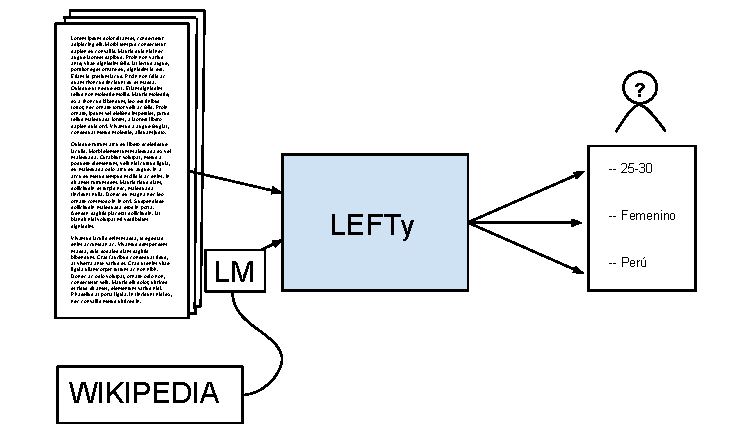
\includegraphics[scale=1.0]{Figures/projectstruct.pdf}
\caption{Estructura del proyecto planteado en este trabajo de investigación. La figura está diseñada para propósitos ilustrativos. \textit{LM} denota el modelo de lenguaje que es pre-entrenado con texto de \textit{Wikipedia} y es un paso previo.}
\label{fig:projstruct}
\end{figure}

La figura \ref{fig:projstruct} muestra la estructura del proyecto planteado, que llenaría los requisitos expuestos en esta sección. El flujo de la información tendría la forma ilustrada en la figura y las predicciones mostradas son ejemplos de categorizaciones.

\section{Resumen}

El proyecto deberá tener la flexibilidad de adaptarse a las necesidades del caso de uso específico que se le dé y a la vez tener la capacidad predictiva de un modelo del estado del arte. El modelo utilizará tecnologías de Deep Learning, por ser la tecnología más prometedora en este campo.





